
\section{Particle Flow Algorithim}

The global event reconstruction (also called particle-flow event reconstruction~\cite{CMS-PRF-14-001}) aims to reconstruct and identify each individual particle in an event, with an optimized combination of all subdetector information. In this process, the identification of the particle type (photon, electron, muon, charged hadron, neutral hadron) plays an important role in the determination of the particle direction and energy. Photons ($e/\gamma$ coming from $Z$ decays or from electron bremsstrahlung) are identified as ECAL energy clusters not linked to the extrapolation of any charged particle trajectory to the ECAL. Electrons are identified as a primary charged particle track and potentially many ECAL energy clusters corresponding to this track extrapolation to the ECAL and to possible bremsstrahlung photons emitted along the way through the tracker material. Muons are identified as tracks in the central tracker consistent with either a track or several hits in the muon system, and associated with calorimeter deposits compatible with the muon hypothesis. Charged hadrons are identified as charged particle tracks neither identified as electrons, nor as muons. Finally, neutral hadrons are identified as HCAL energy clusters not linked to any charged hadron trajectory, or as a combined ECAL and HCAL energy excess with respect to the expected charged hadron energy deposit. Figure~\ref{cms_particle_flow} show the identification process for each high-level physics object, as previously described.


% cms particle flow
\begin{figure}[htbp]
    \centering
    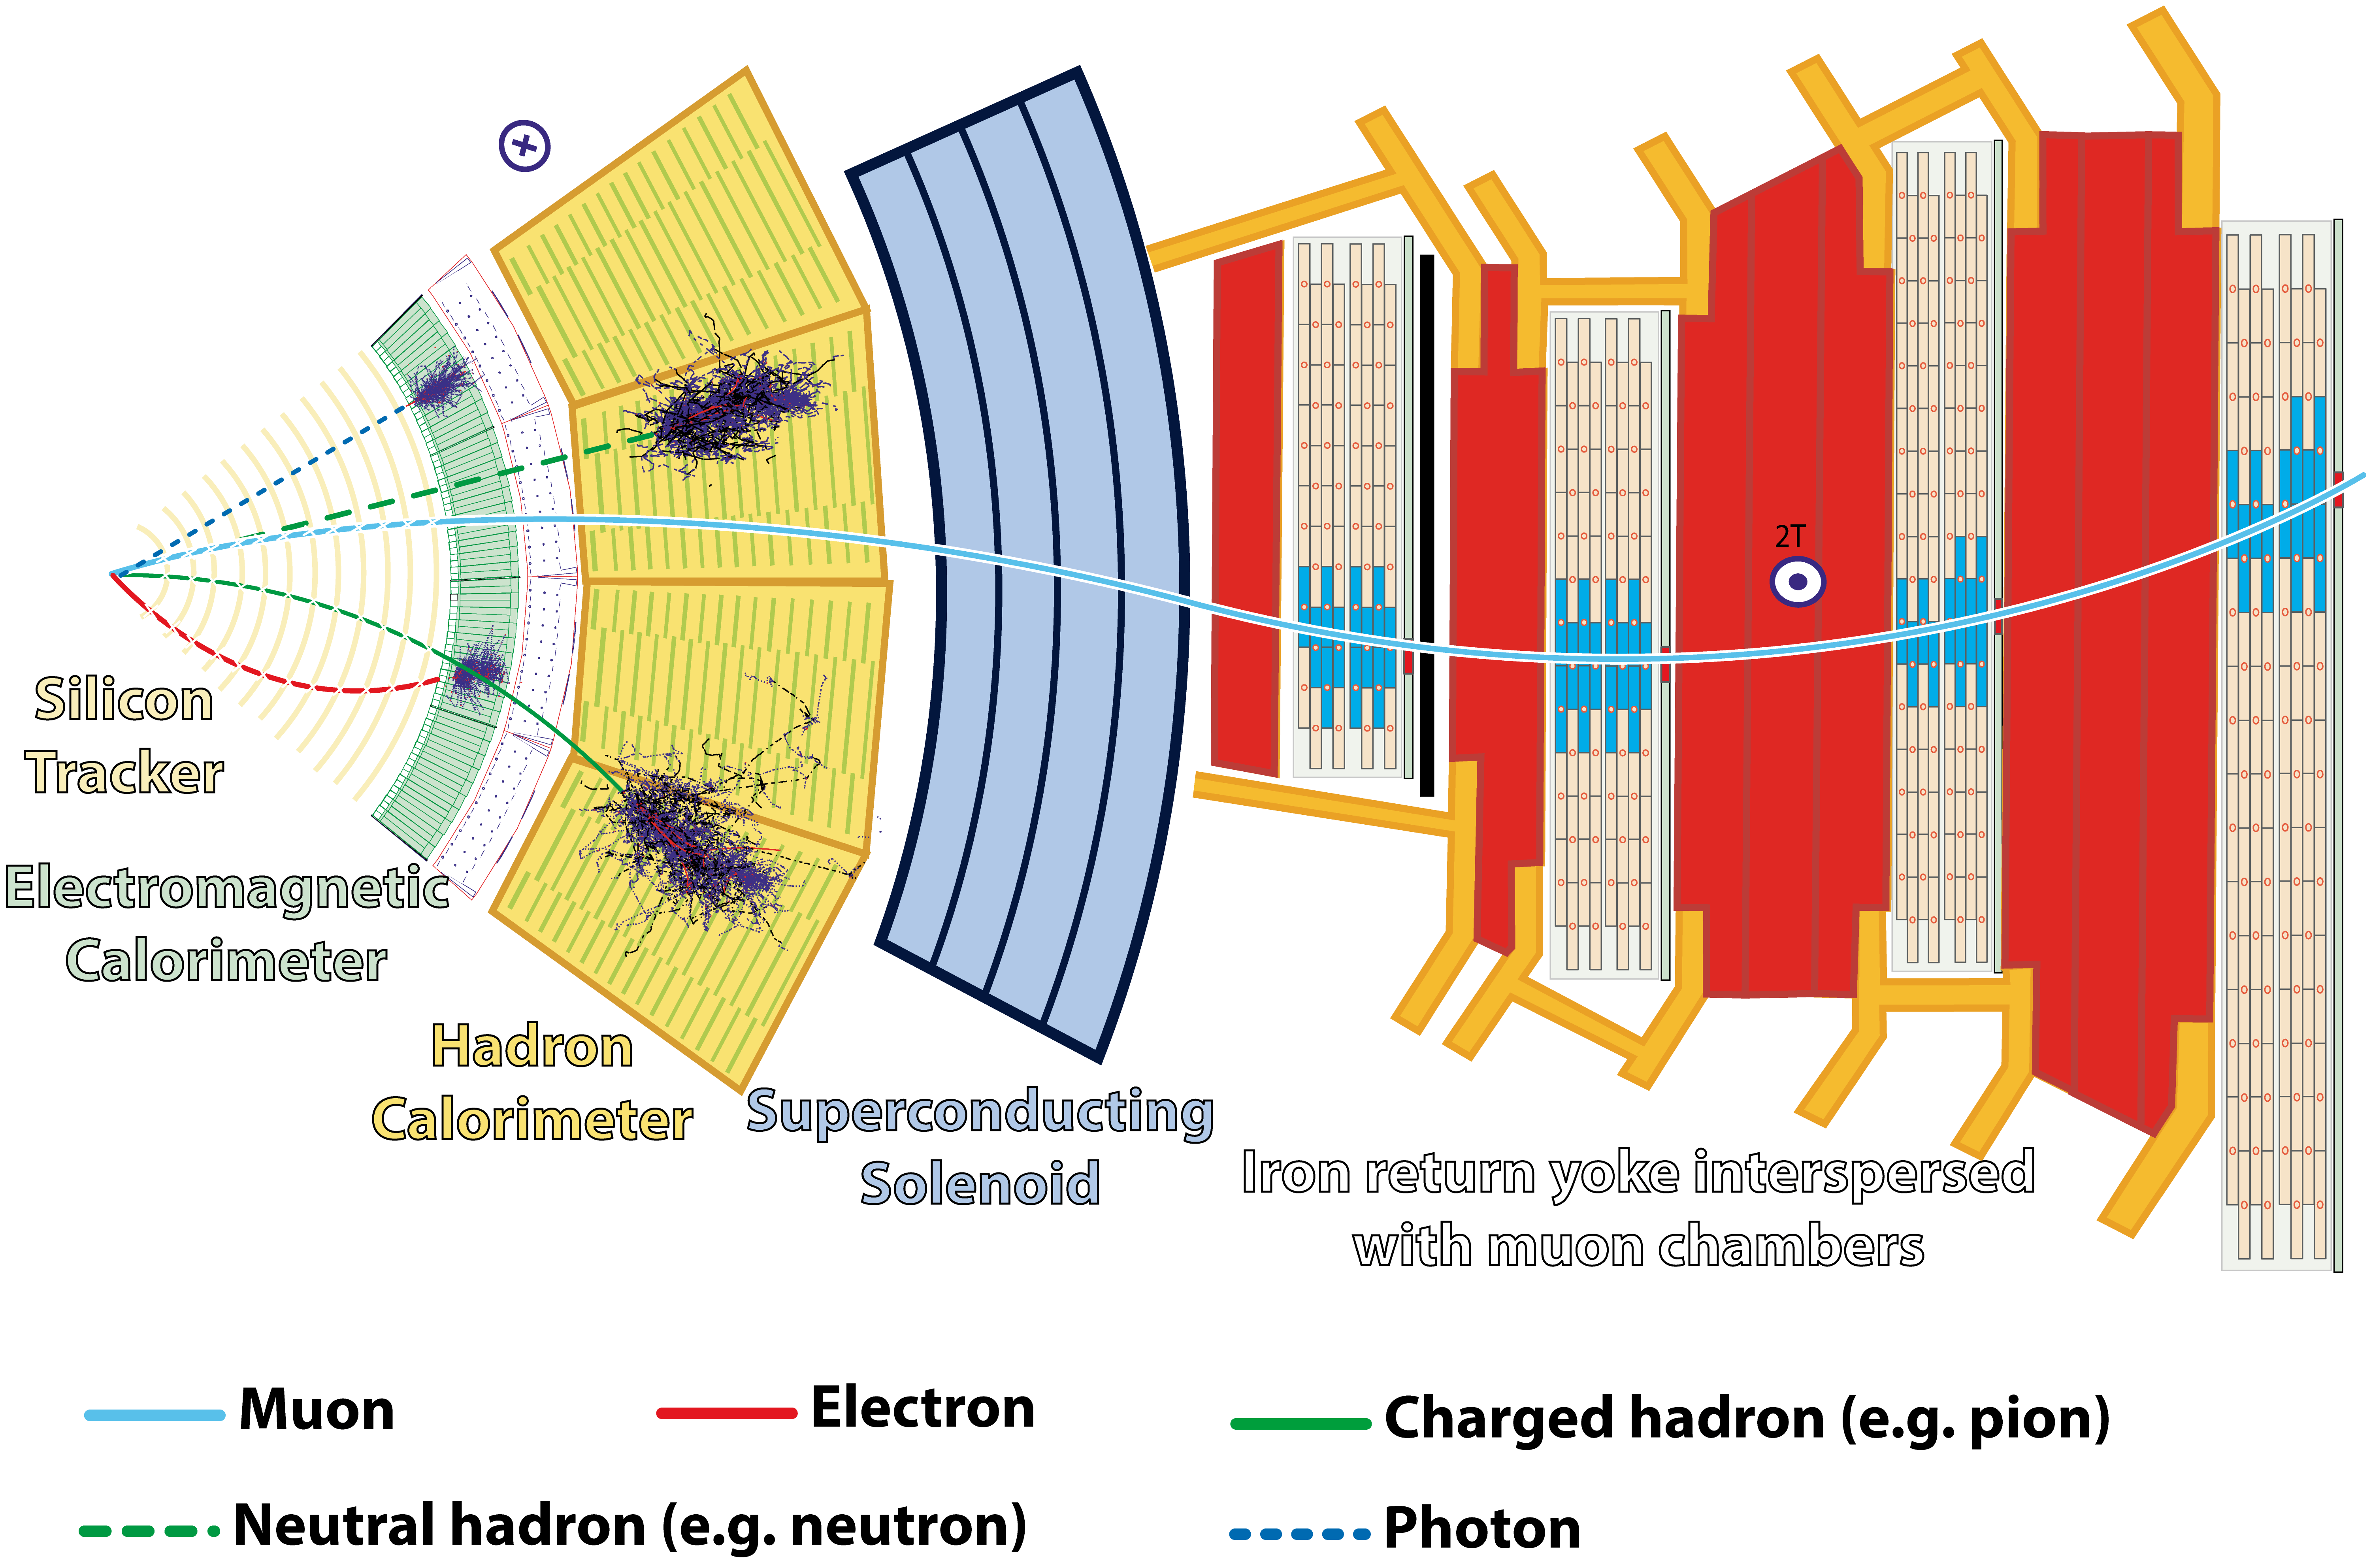
\includegraphics[width=0.7\textwidth]{figures_and_tables/experimental_setup/particle_flow.png}
    \caption{The figure illustrates how the information from each subdetector is used in order to identify the different high-level objects in the Particle-Flow algorithm. Source:~\cite{CMS-PRF-14-001}.}
    \label{cms_particle_flow}
\end{figure}

The energy of photons is obtained from the ECAL measurement. The energy of electrons is determined from a combination of the track momentum at the main interaction vertex, the corresponding ECAL cluster energy, and the energy sum of all bremsstrahlung photons attached to the track. The energy of muons is obtained from the corresponding track momentum. The energy of charged hadrons is determined from a combination of the track momentum and the corresponding ECAL and HCAL energies, corrected for the response function of the calorimeters to hadronic showers. Finally, the energy of neutral hadrons is obtained from the corresponding corrected ECAL and HCAL energies.

The candidate vertex with the largest value of summed physics-object $\pt^2$ is taken to be the primary $pp$ interaction vertex. For each event, hadronic jets are clustered from these reconstructed particles using the infrared and collinear safe anti-\kt algorithm~\cite{Cacciari:2008gp, Cacciari:2011ma} with a distance parameter of 0.4. Jet momentum is determined as the vectorial sum of all particle momenta in the jet, and is found from simulation to be, on average, within 5 to 10\% of the true momentum over the whole \pt spectrum and detector acceptance. Additional proton-proton interactions within the same or nearby bunch crossings (pileup) can contribute additional tracks and calorimetric energy depositions to the jet momentum. To mitigate this effect, charged particles identified to be originating from pileup vertices are discarded and an offset correction is applied to correct for remaining contributions. Jet energy corrections are derived from simulation to bring the measured response of jets to that of particle level jets on average. In situ measurements of the momentum balance in dijet, $\text{photon} + \text{jet}$, $Z + \text{jet}$, and multijet events are used to account for any residual differences in the jet energy scale between data and simulation~\cite{Khachatryan:2016kdb}. The jet energy resolution amounts typically to 15--20\% at 30\GeV, 10\% at 100\GeV, and 5\% at 1\TeV~\cite{Khachatryan:2016kdb}. Additional selection criteria are applied to each jet to remove jets potentially dominated by anomalous contributions from various subdetector components or reconstruction failures.

Anomalous high-\ptmiss events can be due to a variety of reconstruction failures, detector malfunctions or non collisions backgrounds. Such events are rejected by event filters that are designed to identify more than 85--90\% of the spurious high-\ptmiss events with a mistagging rate less than 0.1\%~\cite{Sirunyan:2019kia}.

Hadronic decays of top quarks are identified using the ratio between 3-subjettiness and 2-subjettiness~\cite{Thaler:2010tr}, $\tau_{32}=\tau_{3}/\tau_{2}$, and the groomed jet mass. The groomed jet mass is calculated after applying a modified mass-drop algorithm~\cite{Dasgupta:2013ihk,Butterworth:2008iy}, known as the \emph{soft drop} algorithm~\cite{Larkoski:2014wba}, to anti-\kt jets with a distance parameter of 0.8 and parameters $\beta=0$, $z_\text{cut}=0.1$, and $R_0 = 0.8$. The variables are calibrated in a top quark-antiquark enriched sample~\cite{Sirunyan:2020foa}.

In the barrel section of the ECAL, an energy resolution of about 1\% is achieved for unconverted or late-converting photons in the tens of \GeV energy range. The remaining barrel photons have a resolution of about 1.3\% up to a pseudorapidity of $\abs{\eta} = 1$, rising to about 2.5\% at $\abs{\eta} = 1.4$. In the endcaps, the resolution of unconverted or late-converting photons is about 2.5\%, while the remaining endcap photons have a resolution between 3 and 4\%~\cite{CMS:EGM-14-001}.

The electron momentum is estimated by combining the energy measurement in the ECAL with the momentum measurement in the tracker. The momentum resolution for electrons with $p_T \approx 45$ GeV from $\Z \rightarrow ee$ decays ranges from 1.7\% to 4.5\%. It is generally better in the barrel region than in the endcaps, and also depends on the bremsstrahlung energy emitted by the electron as it traverses the material in front of the ECAL~\cite{Khachatryan:2015hwa}.

Muons have their momentum computed by curvature of their tracks in the muon system solo or the matched track in the muon system and the tracker.